\subsection{Introduction}

Some properties are such that it's possible to check whether they're true or false simply by computation. These properties are called \emph{decidable}, and in Coq we can describe the decidable propositions with the algebraic data type
\[
\mathsf{Decidable}\ (P : \Prop) : \Type \triangleq
  \begin{cases}
  \mathsf{Yes}\ (y : P) : \mathsf{Decidable}\ P
  \\ \mathsf{No}\ (n : \neg P) : \mathsf{Decidable}\ P
  \end{cases}.
\]

Decidable propositions are closed under many logical operations, such as finite conjunctions and disjunctions. That is, if $P$ and $Q$ are both decidable, then so are $P \wedge Q$ and $P \vee Q$. And we can state this property in another way as well. If we have $A : \Type$ and $P : A \to \Prop$, we say $P$ is a decidable predicate if $\prod_{a : A} \mathsf{Decidable}\ (P\ a)$ holds. Then, if $A$ is Kuratowski-finite (i.e., there is some $\ell : \mathsf{list}\ A$ such that every element of $A$ is in that list) and $P$ is a decidable predicate on $A$, the propositions $\forall a : A, P\ a$ and $\exists a : A, P\ a$ are also decidable.

Sometimes in formal verification, we are lucky and it turns out that properties of interest turn out to be decidable. In this case, verification consists of very little work, for humans at least, because we can simply run a computer program to determine whether or not the proposition is true.

When we move to the continuous world, it at first seems that we are less lucky, because so many predicates are undecidable. For instance, determining whether one real number is less than another is undecidable. Additionally, very few spaces have sets of points which are Kuratowski-finite, and many spaces of interest aren't even countable; for instance, the real numbers are (potentially) uncountable.

I'd like to advance the argument that the notions of ``decidable propositions'' and ``Kuratowski-finite sets'' should be generalized to \emph{binary covers} and \emph{compact/overt spaces}. The convenient properties about decidable reasoning over finite sets then largely carries over to these generalized notions for topological spaces.

We'll start by back-translating what binary covers ought to mean just in the world of Coq's sets and propositions. Note that there's an asymmetry in the definition of $\mathsf{Decidable}$, to a constructive reader, at least, in considering $P$ and $\neg P$ as opposites. Of course, for decidable propositions, this is okay, because here everything looks classical, and so they are in fact opposites. Similarly, we have
\[
\neg \left( \exists x : A, \forall y : B, \exists z : C, P(x, y, z) \right) = \forall x : A, \exists y : B, \forall z : C, \neg P(x, y, z)
\]
when $A$, $B$, and $C$ are finite and when $P$ is a decidable predicate. That is, we see that the $\exists$ and $\forall$ quantifiers become opposites, which are flipped by negation. In particular, we have
\[
\mathsf{Decidable}\ P \leftrightarrow \mathsf{Decidable}\ (\neg P),
\]
so there's no reason to think of $P$ as the ``true'' thing and $\neg P$ as the ``false'' thing. We're just choosing between two mutually exclusive alternatives. A binary cover weakens this, by not requiring that the two alternatives be mutually exclusive. So a binary cover represents a decision, but it might happen to be the case that both decisions are mutually permissible.

In the world of Coq, a pair of propositions $\langle P, Q \rangle$ is a binary cover if the algebraic datatype $\mathsf{BCover}\ P\ Q$ holds, which is defined as
\[
\mathsf{BCover}\ (\langle P, Q \rangle : \Prop \times \Prop) : \Type \triangleq
  \begin{cases}
  \mathsf{Left}\ (\ell : P) : \mathsf{BCover}\ P\ Q
  \\ \mathsf{Right}\ (r : Q) : \mathsf{BCover}\ P\ Q
  \end{cases}.
\]

We can define logical operations on these pairs of propositions which generalizes the logical connectives for single propositions, where we consider the first proposition normally and the second in reverse:
\begin{align*}
\langle P_1, Q_1 \rangle \Rightarrow \langle P_2, Q_2 \rangle
\qquad &\triangleq \qquad 
(P_1 \Rightarrow P_2) \wedge (Q_2 \Rightarrow Q_1)
\\
\langle P_1, Q_1 \rangle \wedge \langle P_2, Q_2 \rangle
\qquad &\triangleq \qquad 
\langle P_1 \wedge P_2, Q_2 \vee Q_1 \rangle
\\
\langle P_1, Q_1 \rangle \vee \langle P_2, Q_2 \rangle
\qquad &\triangleq \qquad 
\langle P_1 \vee P_2, Q_2 \wedge Q_1 \rangle
\\
\neg \langle P, Q \rangle
\qquad &\triangleq \qquad 
\langle Q, P \rangle
\\
\forall_A \langle P, Q \rangle
\qquad &\triangleq \qquad 
\langle \forall a : A, P(a) , \exists a : A, Q(a) \rangle
\\
\exists_A \langle P, Q \rangle
\qquad &\triangleq \qquad 
\langle \exists a : A, P(a) , \forall a : A, Q(a) \rangle
\end{align*}
Note that the logical connectives on the right-hand side of the definitions are the regular logical connectives on Coq propositions, while the ones on the left-hand side are being defined for pairs of propositions (and predicates). The definition of $\Rightarrow$ on pairs of propositions determines a preorder, with a top element $\langle \top, \bot \rangle$ and a bottom element $\langle \bot, \top \rangle$, and equivalence given by
\[
\langle P_1, Q_1 \rangle \Leftrightarrow \langle P_2, Q_2 \rangle
\qquad \triangleq \qquad 
(P_1 \Leftrightarrow P_2) \wedge (Q_1 \Leftrightarrow Q_2)
\]

Just as decidable propositions/predicates are closed under finite conjunction and disjunction and quantification over finite sets, so are binary covers closed under those similar generalized operations which were defined above. There is additionally the analogous symmetry for flipping a decision,
\[
\mathsf{BCover}\ U \leftrightarrow \mathsf{BCover}\ (\neg U).
\]

There are, of course, some differences, too. The most important one is that if there are two deciders for a proposition $P$, then they either both answer $\mathsf{Yes}$ or they both answer $\mathsf{No}$, because those possibilities are disjoint. However, this is patently untrue for pairs of propositions. For the pair of propositions $\langle \top, \top \rangle$, we can inhabit $\mathsf{BCover}\ \langle \top, \top \rangle$ both with $\mathsf{Left}$ as well as $\mathsf{Right}$.

We can also define a new relation on pairs of propositions called the \emph{specialization order}, defined by
\[
\langle P_1, Q_1 \rangle \le \langle P_2, Q_2 \rangle
\qquad \triangleq \qquad 
(P_1 \Rightarrow P_2) \wedge (Q_1 \Rightarrow Q_2).
\]
As the name and notation suggest, the specialization order indeed forms a preorder. An important but obvious fact about the specialization order is that if $U \le V$, then $\mathsf{BCover}\ U \to \mathsf{BCover} \ V$. That is, if we can make a decision about $U$, then we can also make a decision about $V$.

There is a maximal pair of propositions for the specialization order, $\langle \top, \top \rangle$, for which it is very easy to make decisions. If we restrict to pairs of propositions which are in fact binary covers, then there is no minimal binary cover (with respect to the specialization order).

\subsection{Binary covers for spaces}

We can quite mechanically translate our definitions over from Coq to \textbf{Top}. Instead of propositions, we consider the Sierp\'inski space $\Sigma$. Here, we can define the space $\mathsf{BCover}$ as the open subspace
\[
\mathsf{BCover} \triangleq \{ (P, Q) : \Sigma \times \Sigma \suchthat P \vee Q \}
\]
of the product of $\Sigma$ with itself. Let's define $\mathsf{Left} : \Open{A}$ as $\mathsf{Left} \triangleq \mathsf{strict} \times \top_\Sigma$, the open subspace where the first projection is $\mathsf{true}$, and $\mathsf{Right} \triangleq \top_\Sigma \times \mathsf{strict}$. Then, in a ``point-free'' notation, we could have equivalently defined
\[
\mathsf{BCover} \triangleq \{ \Sigma \times \Sigma \suchthat \mathsf{Left} \vee \mathsf{Right} \}.
\]
Then a continuous map $f : A \to \mathsf{BCover}$ from some space $A$ is the same as an open cover of the space $A$ comprised of two open sets.  Given $f$, the open cover is given by $f^{-1}(\mathsf{Left})$ and $f^{-1}(\mathsf{Right})$, and we can derive
\begin{align*}
f^{-1}(\mathsf{Left}) \vee f^{-1}(\mathsf{Right})
\tag{$f^{-1}$ preserves arbitrary suprema}
&= f^{-1}(\mathsf{Left} \vee \mathsf{Right})
\\ &\ge f^{-1}\left (\top_\mathsf{BCover} \right)  \tag{$f^{-1}$ monotonic, defn. of $\mathsf{BCover}$ as open subspace}
\\ &= \top_A, \tag{$f^{-1}$ preserves $\top$}
\end{align*}
that is,
\[
\top_A \le f^{-1}(\mathsf{Left}) \vee f^{-1}(\mathsf{Right}),
\]
meaning that this indeed gives a binary cover of $A$.

Given a binary cover of $A$, i.e., opens $U$ and $V$ of $A$ such that $\top_A \le U \vee V$, it is likewise possible to construct a continuous map $f: A \to \mathsf{BCover}$, by the same argument (played in reverse).

What are the (global) points of $\mathsf{BCover}$? Since there are two global points of the Sierp\'inski space $\Sigma$, $\mathsf{true}$ and $\mathsf{false}$, there are four points of $\Sigma \times \Sigma$, and three of them lie in the open subspace $\mathsf{BCover}$: $(\mathsf{true}, \mathsf{false}), (\mathsf{true}, \mathsf{true}),$ and $(\mathsf{false}, \mathsf{true})$. Let's name these points $\mathsf{L}$, $\mathsf{B}$, and $\mathsf{R}$, respectively. In the scenario where one of the points is $\mathsf{false}$, then the computational behavior of the point is determined: given the non-trivial open cover asking which open holds, there's only one possibility. But for the point $\mathsf{B} = (\mathsf{true}, \mathsf{true})$, there are two possibilities: that is, two implementations of the same point $\mathsf{B}$ can behave differently, just as there are two computationally different inhabitants of the Coq type $\mathsf{BCover}\ \langle \top, \top \rangle$.

For topological spaces, we automatically get a notion of specialization order on points of a space, and the specialization order on points of $\mathsf{BCover}$ agrees with our earlier definition of specialization order on pairs of Coq propositions. Just as we observed with Coq pairs of propositions that if $U \le V$, then $\mathsf{BCover}\ U \to \mathsf{BCover}\ V$, we have a fundamental property for specialization order of points. For two points $x$ and $y$ of a space $A$, if $x \le y$, then $y$ may always ``behave'' computationally exactly as $x$. That is, the computational behavior of $x$ can be used to produce computational behavior of $y$.

In particular, for our three points of $\mathsf{BCover}$, we get the following Hasse diagram for the specialization order:
\begin{center}
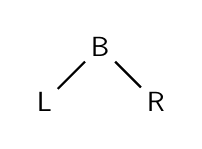
\begin{tikzpicture}
    \node (top) at (0,0) {$\mathsf{B}$};
    \node [below left  of=top] (left)  {$\mathsf{L}$};
    \node [below right of=top] (right) {$\mathsf{R}$};

    % Now draw the lines:
    \draw [thick, shorten <=-2pt, shorten >=-2pt] (top) -- (left);
    \draw [thick, shorten <=-2pt, shorten >=-2pt] (top) -- (right);
\end{tikzpicture}
\end{center}

What's interesting to note is that the points of $\mathsf{BCover}$ always have maxima with respect to specialization order. That means it's always possible to non-deterministically join points of $\mathsf{BCover}$ together.

Just as we found that the ``conjunction'' and ``disjunction'' operations of pairs of Coq propositions preserved having binary covers, we can define continuous maps representing conjunction and disjunction over the $\mathsf{BCover}$ space:
\begin{align*}
\cdot \wedge \cdot &: \mathsf{BCover} \times \mathsf{BCover} \to \mathsf{BCover}
\\ x \wedge y &\triangleq \mathsf{cases}(x, y)
\begin{cases}
\mathsf{Left}, \mathsf{Left}
 \qquad &\Rightarrow \qquad
 \mathsf{L}
\\
\mathsf{Right}, \_\_
 \qquad &\Rightarrow \qquad
 \mathsf{R}
\\
\_\_, \mathsf{Right}
 \qquad &\Rightarrow \qquad
 \mathsf{R}
\end{cases}
\\
\cdot \vee \cdot &: \mathsf{BCover} \times \mathsf{BCover} \to \mathsf{BCover}
\\ x \vee y &\triangleq \mathsf{cases}(x, y)
\begin{cases}
\mathsf{Left}, \_\_
 \qquad &\Rightarrow \qquad
 \mathsf{L}
\\
\_\_, \mathsf{Left}
 \qquad &\Rightarrow \qquad
 \mathsf{L}
\\
 \mathsf{Right}, \mathsf{Right}
 \qquad &\Rightarrow \qquad
 \mathsf{R}
\end{cases}.
\end{align*}

Are these definitions, using overlapping pattern matching, valid definitions? There are two conditions to check: that the cases cover the entire input space, and that overlapping branches have a maximum in terms of specialization order. Since the output space is $\mathsf{BCover}$, which always maxima, we always satisfy the second condition. Since we have the cover
\[
\top_\mathsf{BCover} \le \mathsf{Left} \vee \mathsf{Right},
\]
we have in the product space
\begin{align*}
\top_{\mathsf{BCover} \times \mathsf{BCover}} \le 
  &(\mathsf{Left} \times \mathsf{Left}) \vee (\mathsf{Left} \times \mathsf{Right})
\\ \vee &(\mathsf{Right} \times \mathsf{Left}) \vee (\mathsf{Right} \times \mathsf{Right}),
\end{align*}
which clearly shows that the cases in the definitions of conjunction and disjunction also cover the entire input space.

It's still important to check that these definitions satisfy the definitions you'd expect for conjunction and disjunction on binary covers. Negation is easy as well:
\begin{align*}
 \neg &: \mathsf{BCover} \to \mathsf{BCover}
\\ \neg x &\triangleq \mathsf{cases}(x)
\begin{cases}
\mathsf{Left}
 \qquad &\Rightarrow \qquad
 \mathsf{R}
\\
\mathsf{Right}
 \qquad &\Rightarrow \qquad
 \mathsf{L}
\end{cases}
\end{align*}

If you're bothered by the fact that the two opens in a binary cover get ``opposite'' treatments, and in particular that the logical operations on the second open are in reverse, for no good reason, there's another way to think about it. Rather than thinking of a binary cover of $A$ as two opens $P, Q : \Open{A}$ such that $A \subseteq P \cup Q$, we can instead think of it as an open set $P$ and a \emph{closed} set $\overline{Q}$ which is the ``set-theoretic'' complement of $Q$, since the complement of an open set is closed. Then the fact that $\langle P, Q \rangle$ is a binary cover means that $\overline{Q} \subseteq P$. Then the definitions of the logical operations should make more sense. For instance, one can find the union of two closed sets by taking their complement to produce two open sets, taking the intersection of that, and then taking the complement to return to a closed set. Since we are simply ``encoding'' closed sets with their open complements, computing the ``union'' just corresponds to taking an intersection.

This elicits the view of binary covers as ``approximate'' predicates, sandwiching a closed subspace inside an open one, with wiggle room for for points which are in between. Any points which are in $\overline{Q}$ (and thus also $P$) will definitely compute to $\mathsf{Left}$, while any points which are outside of $P$ (and thus also outside $\overline{Q}$ will definitely compute to $\mathsf{Right}$, while in-between points, which are in $P$ but not $\overline{Q}$, are allowed to compute either way.

\subsection{Binary covers on $\R$}

The decidable predicates on a Coq type are analogous in \textbf{Top} to \emph{disconnections} or \emph{separations} of a space $A$, which are fancy terms for continuous maps $A \to \bool$ (just as decidable predicates on a type $A$ in Coq correspond to functions from $A$ to $\bool$). Equivalently, these are decompositions of a space into two disjoint opens. For the real numbers, $\R$, the only separation is the trivial one, where one open is the entire space, $\top_\R$, and the other the empty space, $\bot_\R$. When the only separations are trivial, in the case of $\R$, the space is called \emph{connected}, whose name accurately conveys the intuition of this notion for most spaces.

While there's a paucity of separations for $\R$, there is a wealth of binary covers, making it possible to ``do logic'', in a computable way (similarly as with decidable propositions), on $\R$. It's hard to exhaust all of them, but we can consider a particularly interesting class of them. For any tolerance $\varepsilon : \rat^+$, there is the map $\cdot <_\varepsilon \cdot : \R \times \R \to \mathsf{BCover}$ which satisfies for all $x, y : \R$
\begin{align*}
x <_\varepsilon y \models \mathsf{Left} 
\qquad &\Leftrightarrow \qquad
x < y
\\
x <_\varepsilon y \models \mathsf{Right} 
\qquad &\Leftrightarrow \qquad
x > y - \varepsilon,
\end{align*}
yielding an ``approximate'' comparison with error up to $\varepsilon$. Notice the intentional asymmetry in the definition here. We are setting up our our $\mathsf{BCovers}$ on $\R$ such that if an $\varepsilon$-approximate proposition ``computes'' that it lies in $\mathsf{Left}$, then it indeed lies in that open set indicated by the approximate proposition, while if it computes to $\mathsf{Right}$, it either doesn't lie in the indicated open, or it is ``barely inside'' the open, no more than $\varepsilon$ away from the border. However, this interpretation relies on never using the negation operator, since negation swaps these roles.

Just this $\R$-specific comparison operator is enough to reproduce all the logical operations of dReal, together with their computational meaning. dReal also offers a predicate $\cdot \le_\varepsilon \cdot$, which is useless, since it is identical to $\cdot <_\varepsilon \cdot$.

\subsection{Compactness}

In the world of Coq, we observed if a predicate $P$ on a set $A$ is decidable and if $A$ is Kuratowski-finite, then $\forall a : A, P(a)$ and $\exists a : A, P(a)$ are decidable as well. The analog of this for \textbf{Top} are the compact/overt spaces.

[cite nLab]
A space $A$ is \emph{compact} if for every space $\Gamma$, and every open $U : \Open{\Gamma \times A}$, there is an open $\forall_A U : \Open{\Gamma}$ such that for every $V : \Open{\Gamma},$
\[
V \le_\Gamma \forall_A U \qquad \Leftrightarrow \qquad \top_A \times V \le_{\Gamma \times A} U.
\]
Similarly, a space $A$ is \emph{overt} if for every space $\Gamma$, and every open $U : \Open{\Gamma \times A}$, there is an open $\exists_A U : \Open{\Gamma}$ such that for every $V : \Open{\Gamma},$
\[
\exists_A U \le_\Gamma V  \qquad \Leftrightarrow \qquad U  \le_{\Gamma \times A} \top_A \times V.
\]

These conditions are the definitions of universal and existential quantification in terms of adjoints, viewing $\Gamma$ as some context and opens as truth values in a context.

A \emph{compact/overt} space is a space which is both compact and overt. Now, suppose we have a compact/overt space $A$ which has opens $P, Q : \Open{A}$ which are a binary cover, i.e.,
\[
\top_A \le P \vee Q.
\]

To universally quantify over this binary cover, we'd like to show that
\[
\top_\Sigma \le \forall_A P \vee \exists_A Q,
\]
which follows from the derivation
\begin{align*}
\top_\Sigma 
  &\le \forall_A (\top_A)
\\ &\le \forall_A(P \vee Q)  \tag{since $\top_A \le P \vee Q$}
\\ &\le \forall_A P \vee \exists_A Q.
\end{align*}

Similarly, we can existentially quantify over the binary cover compose of $P, Q : \Open{A}$ to produce the binary cover
\[
\top_\Sigma \le \exists_A P \vee \forall_A Q,
\]
in a completely symmetric manner.

If we expand to work in the gros topos, where we have higher order functions, these functions for quantification, which allow us to extend quantification over opens to quantification over $\mathsf{BCover}$s, give us the operations $\forall_A : (A \to \mathsf{BCover}) \to \mathsf{BCover}$ and $\exists_A : (A \to \mathsf{BCover}) \to \mathsf{BCover}$ if $A$ is compact/overt.\footnote{Note that if $A$ is only compact or only overt, neither are possible, since the ``opposite'' quantification is used on the ``right'' side.}

Compact and overt subspaces of a space are closed under finitary union and intersection, so compact/overt subspaces are also closed under finite union and intersection. Additionally, the continuous image of a compact space is compact (just as the image of a finite space is finite), and likewise for overt spaces, so the continuous image of a compact/overt space is compact/overt.

For the real numbers, we have that for any real numbers $a, b : \R$ such that $a < b$, the closed interval from $a$ to $b$ is compact/overt. Of course, we can then take unions and intersections of intervals and still have compact/overt subspaces. This corresponds to the fact that dReal is able to quantify over intervals of $\R$.

\subsection{Non-determinism}

The generalization of decidable propositions to binary covers, and of finite sets to compact/overt spaces, should give us hope that exhaustive reasoning over continuous spaces is possible in many real-world scenarios, in particular because there ought to be plenty of useful binary covers and compact/overt spaces for verification tasks. The fact that the continuous image of a compact/overt space is compact/overt means that, as long as the space of inputs is compact/overt, and the query about the outputs is a binary cover, it is possible to just compute an answer to the query.

However, there's an issue with this line of argument, which is that continuous systems often make discrete decisions over continuous spaces. In order to do this, their decisions are necessarily non-deterministic. What this means is that rather than the output being some space $A$, which we might imagine to be a nice space, it is $\PLower(A)$, the space of overt subspaces of $A$. Since overt subspaces are not (in general) compact, we cannot simply quantify over $\PLower(A)$, even though this is what we'd like to do. For instance, we might want to know whether our autonomous car stays in our ``safe region'' for every non-deterministic choice it might make, or whether it is close to leaving that ``safe region'' in any non-deterministic choice it might make.

This issue is quite fundamental. Let's consider a simple example of how significant it is to change the output space from $A$ to $\PLower(A)$. Let's consider functions from the closed unit interval $[0,1]$ to $\R$. Any continuous map $f : [0,1] \to \R$ must be bounded, since the continuous image of a compact space is compact. Intuitively, there's no room for the graph of $f$ to ``escape'' and do anything weird:

\begin{center}
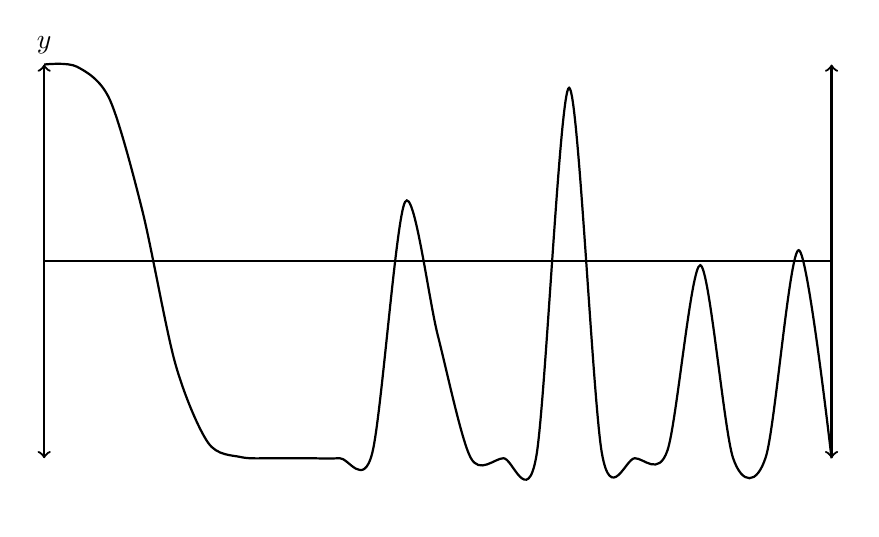
\begin{tikzpicture}[scale=2.5]
\draw[thick] (0,0) -- (4,0) node[right] {};
\draw[<->, thick] (0,-1) -- (0,1) node[above] {$y$};
\draw[<->, thick] (4,-1) -- (4,1);
\draw[scale=1,domain=0:4,smooth,thick,variable=\x] plot ({\x},{2*exp(-10*(sin(50*\x*\x))^2)-1});
\end{tikzpicture}
\end{center}

However, as soon as we allow non-determinism, we can do funky things. Here's a map $f : [0,1] \to \PLower(\R)$ which always maps each input to at most two outputs. Still, we see that $f$ no longer need be bounded:
\begin{center}
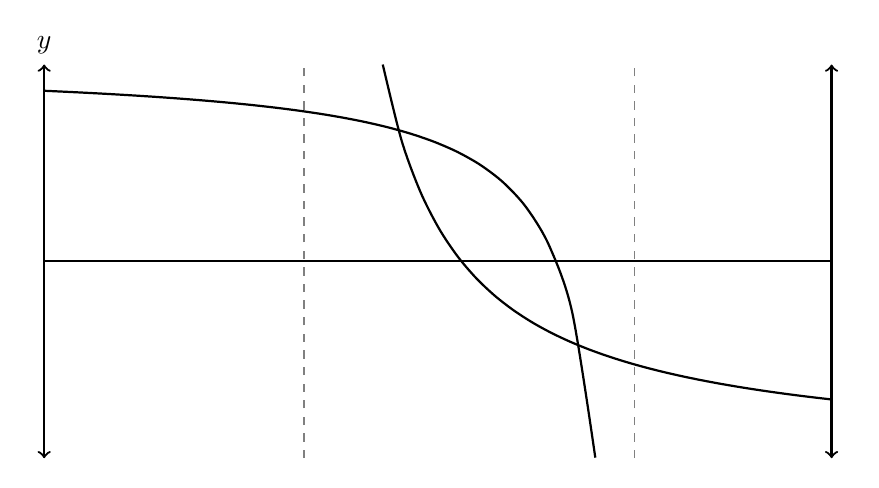
\begin{tikzpicture}[scale=2.5]
\draw[thick] (0,0) -- (4,0) node[right] {};
\draw[<->, thick] (0,-1) -- (0,1) node[above] {$y$};
\draw[<->, thick] (4,-1) -- (4,1);
\draw[scale=1,domain=0:2.8,smooth,thick,variable=\x] plot ({\x},{1 + 0.1/(0.25*(\x - 2) - 0.25))});
\draw[dashed, gray] (3,-1) -- (3,1);
\draw[scale=1,domain=1.72:4,smooth,thick,variable=\x] plot ({\x},{-1 + 0.2/(0.25*(\x - 2) + 0.17))});
\draw[dashed, gray] (1.32,-1) -- (1.32,1);
\end{tikzpicture}
\end{center}

Even though this is constructed from a non-deterministic merge of two deterministic cases, its behavior is potentially unbounded, because each of those cases is defined on an open subspace which in this case is not compact.

Another way in which nondeterminism can break compactness is by having a non-deterministic merging of infinitely many compact sets. For instance, consider
\begin{align*}
f &: [0,1] \to \PLower(\R)
\\ f(x) &\triangleq \mathsf{cases}(x)
\begin{cases}
[n : \nat] \quad &\cdot > 1 / n
 \qquad \Rightarrow \qquad
 \{ n \}
\\ \quad &\cdot < 1/2
\qquad \Rightarrow \qquad
\{ 0 \}
\end{cases}
\end{align*}

When \emph{can} we admit exhaustive reasoning, then, for continuous maps of the form $A \to \PLower(B)$, where $A$ is compact? The first issue was that maps defined on an open space might not be bounded. One possible solution to this is to demand that each branch of a $\mathsf{cases}$ expression admit a continuous extension to a compact space. That is, suppose one of the branches is of the form $f : U \to \mathcal{P}(B)$, where $U$ is open and $\mathcal{P}(B)$ represents the space of compact/overt subspaces of $B$. Then $f$ admits a continuous extension to a compact space if there is some space $C$ which is compact/overt together with maps $i : U \to C$ and $g : C \to \mathcal{P}(B)$ such that $f = g \circ i$. Then, we have that $g(C) : \mathcal{P}(B)$ is compact/overt, and also that $f(U) \subseteq g(C)$, which means that we can \emph{soundly} reason about $f(U)$ by instead reasoning about $g(C)$. However, since $g(C)$ is in general larger than $f(U)$, it might not be the ``tightest'' reasoning that's possible.

For example, consider one of the branches of the map depicted above, which has the vertical asymptote. One of them is defined on the domain $(1/3, 1]$, which is not compact, and so it ``escapes'' off to $+\infty$ as it nears 1/3. This means that it will \emph{not} admit any continuous extension, as long as the codomain is kept as $\R$. By requiring that the branches of a $\mathsf{cases}$ expression admit continuous extensions to compact spaces, it prevents this kind of behavior. If the branch didn't have a vertical asymptote, we'd be able to extend it to the domain $[1/3, 1]$ which is compact/overt. We'd also be able to extend it to $[0,1]$ as well, in which case there would be many possible continuous extensions, and we could essentially make it behave as we wish in the region near 0. When we then analyzed the original branch, which was only on $(1/3, 1]$, the analysis wouldn't be as good, because of the garbage that we added in the new region.

A second issue was shown with the other map $f : [0,1] \to \PLower(\R)$, which had infinitely many branches. Even though each branch, evaluated at a single input point, was a compact/overt space, the union over the infinitely many branches, which sometimes all overlapped at once, was not necessarily compact. In this case, we had that $f(0) = \nat$, which is not compact in $\R$. A simple ``fix'' for this issue is to require having only finitely many branches.

These two conditions allow us to do some (incomplete) exhaustive reasoning about maps of the form $f : A \to \PLower(B)$, with $A$ compact/overt, which are defined by overlapping pattern matching. Here's the most general form in which I can phrase it. Suppose that $f$ is defined as
\begin{align*}
f &: A \to \PLower(B)
\\
f(x) &\triangleq \mathsf{cases}(x)
\begin{cases}
[i : I] \quad f_i(x) \qquad \Rightarrow \qquad \mathsf{inj}_{\lozenge}(e_i(x))
\end{cases},
\end{align*}
where $\mathsf{inj}_\lozenge : \mathcal{P}(B) \hookto \PLower(B)$ is the subspace inclusion which ``forgets'' compactness, the index set $I : \Type$ is finite, each $f_i : U_i \hookto A$ is an open embedding, and each $e_i : U_i \to \mathcal{P}(B)$ admits a continuous extension $e_i' : C_i \to \mathcal{P}(B)$ where $C_i$ is compact.

We wish that $f(A)$ were a compact/overt space such that we could reason about it, but in general, we only have that $f(A)$ is overt. However, we have that
\[
f(A) \subseteq \bigcup_{i : I} e_i'(C_i).
\]
Note that each $e_i'(C_i)$ is a compact/overt space: since the continuous image of a compact set is compact, we have $e_i'(C_i) : \mathcal{P}(\mathcal{P}(B))$, and by the monadicity of $\mathcal{P}$, we can also consider it as just $\mathcal{P}(B)$. Therefore, the union on the right-hand side is a finite union of compact/overt subspaces of $B$, and so it is also compact/overt. Define $C \triangleq \bigcup_{i : I} e_i'(C_i)$. We can exhaustively reason over $C$ with $\mathsf{BCover}$-valued predicates on $B$. If we have $P : B \to \mathsf{BCover}$, and we find that
\[
\forall_C P \models \mathsf{Left},
\]
then certainly $P^{-1}(\mathsf{Left})$ holds everywhere in $f(A)$. Similarly, if we find that
\[
\exists_C P \models \mathsf{Right},
\]
then certainly $P^{-1}(\mathsf{Right})$ holds everywhere in $f(A)$.